\documentclass[letterpaper, 10pt, conference]{ieeeconf}
\usepackage{algorithm,tikz,pgfplots,balance,caption,multicol,lipsum,bbm,verbatim}
\usepackage{amsmath,balance,multicol,url}
\usepackage{amsmath,graphics}
\usepackage{amssymb} 
\usepackage{nicefrac, multirow}
\usepackage{tikz}
\usepackage{bigstrut}
\setlength\bigstrutjot{3pt}
\usepackage{pgfplots}
\pgfplotsset{compat=newest}
\usepackage{subfig}
\usepackage{textcomp}
\usetikzlibrary{backgrounds}
\numberwithin{equation}{section} \newtheorem{thm}{Theorem}[section]  
\newtheorem{cor}[thm]{Corollary}    % Corollary environment
\newtheorem{lem}[thm]{Lemma}        % Lemma environment
\newtheorem{dfn}[thm]{Definition}        % Lemma environment
\newtheorem{prop}[thm]{Proposition}  % Proposition environment
\newtheorem{rem}[thm]{Remark}  % Proposition environment
\newtheorem{con}[thm]{Conjecture}  % Proposition environment
\newcommand{\cS}{\mathcal{S}}
\newcommand{\cR}{\mathcal{R}}
\newcommand{\cD}{\mathcal{D}}
\newcommand{\cN}{\mathcal{N}}
\newcommand{\ceq}{\ensuremath{\mathrel{\stackrel{\mathrm{def}}{=}}}} 
\DeclareMathOperator*{\argmin}{arg\,min}
\DeclareMathOperator*{\argmax}{arg\,max}
\DeclareMathOperator*{\Var}{Var}
\newcommand{\rd}{{\mathrm d}}
\newcommand{\p}{\partial}
\tikzstyle{every node}=[font=\small]
\usepackage{filemod}
\newcommand{\includetikz}[2]{%
\tikzsetnextfilename{#2}%
    \filemodCmp{#1#2.tikz}{#1tikz/#2.pdf}%
        {\tikzset{external/remake next}}{}%
    \input{#1#2.tikz}%
}

\DeclareMathOperator{\J}{J} 
\DeclareMathOperator{\clamp}{clamp} 
\DeclareMathOperator{\interior}{int} 
\DeclareMathOperator{\D}{D} 
\DeclareMathOperator{\Div}{div} 
\DeclareMathOperator{\Sgn}{Sgn} 
\DeclareMathOperator{\Hom}{Hom} 
\DeclareMathOperator{\rank}{rank} 
\DeclareMathOperator{\Vol}{Vol}
\DeclareMathOperator{\Area}{Area}
\DeclareMathOperator{\dVol}{dVol}
\DeclareMathOperator{\supp}{supp} 
\DeclareMathOperator{\Int}{Int} 
\DeclareMathOperator{\Conv}{Conv} 
\DeclareMathOperator{\Cone}{Cone} 
\DeclareMathOperator{\Ker}{Ker} 
\DeclareMathOperator{\Span}{Span} 
\DeclareMathOperator{\Min}{Min} 
\newcommand{\bone}{\mathbf{1}}
\newcommand{\bC}{\mathbb{C}}
\DeclareMathOperator{\tr}{tr} 
\newcommand{\bR}{\mathbb{R}} 
\newcommand{\bZ}{\mathbb{Z}}
\newcommand{\bbeta}{\boldsymbol{\beta}}
\newcommand{\balpha}{\boldsymbol{\alpha}}
\newcommand{\bE}{\mathbb{E}}
\newcommand{\bV}{\mathbb{V}}
\newcommand{\bI}{\mathbb{I}}
\newcommand{\bQ}{\mathbb{Q}}
\newcommand{\bX}{\mathbb{X}}
\newcommand{\bK}{\mathbb{K}}
\newcommand{\bL}{\mathbb{L}} 
\newcommand{\bB}{\mathbb{B}} 
\newcommand{\bT}{\mathbb{T}} 
\newcommand{\bN}{\mathbb{N}}
\newcommand{\bU}{\mathbb{U}}
\newcommand{\cJ}{\mathcal{J}}
\newcommand{\cI}{\mathcal{I}}
\newcommand{\bS}{\mathbb{S}}
\newcommand{\cL}{\mathcal{L}}
\newcommand{\cF}{\mathcal{F}}
\newcommand{\cH}{\mathcal{H}}
\newcommand{\cU}{\mathcal{U}}
\newcommand{\cK}{\mathcal{K}}
\newcommand{\cB}{\mathcal{B}}
\newcommand{\cV}{\mathcal{V}}
\newcommand{\cZ}{\mathcal{Z}}
\newcommand{\cW}{\mathcal{W}}
\newcommand{\cO}{\mathcal{O}} 
\newcommand{\cC}{\mathcal{C}}
\newcommand{\cT}{\mathcal{T}}
\newcommand{\bF}{\mathbb{F}}
\newcommand{\cA}{\mathcal{A}}
\newcommand{\cM}{\mathcal{M}}
\newcommand{\cG}{\mathcal{G}}
\newcommand{\cKG}{\mathcal{KG}}
\renewcommand{\phi}{\varphi}
\renewcommand{\div}{\mbox{div}}
\newcommand{\ve}{\varepsilon}
\newcommand{\norm}[1]{\lVert #1 \rVert}
\newcommand{\abs}[1]{\left| #1 \right|}
\newcommand{\ov}[1]{\overline{#1}}
\newcommand{\diff}[4]{\left.\left.\frac{\operatorname{d}}{\operatorname{d}#1}\right.^{#2}#3\right|_{#4}}
\renewcommand{\geq}{\geqslant}
\renewcommand{\leq}{\leqslant}
\renewcommand{\ge}{\geqslant}
\renewcommand{\le}{\leqslant}

\newcommand{\furlp}[1]{\colorbox{blue!10}{\href{run:/home/fulong/academia/library/papers/#1.pdf}{D}}}
\newcommand{\furlb}[1]{\colorbox{blue!10}{\href{run:/home/fulong/academia/library/books/#1.pdf}{D}}}
\newcommand{\fcitep}[1]{\cite{#1}\mbox{\furlp{#1}}}
\newcommand{\fciteb}[1]{\cite{#1}\mbox{\furlb{#1}}}
% we can now use cite as before


\title{\LARGE \bf Human-Guided DQN: Using Expert Human Gameplay Data on Atari
2600 Games for Deep Reinforcement Learning}
\author{Daniel Seita \\
University of California, Berkeley\\
Email: seita@berkeley.edu
}

\begin{document}
\maketitle

\begin{abstract}
Deep Reinforcement Learning is arguably the hottest and most popular subfield of
Artificial Intelligence. In large part, this was popularized due to the success
of agents in learning how to play Atari games from scratch, given only the input
screen pixels and the game reward as input.  While there has been substantial
follow-up work on how to improve the Deep Q-Network (DQN) algorithm, there has
not been much focus on how to utilize human guidance. In this paper, we report
progress about an idea for using human expert gameplay on Atari games to boost
DQN. During the exploration stage for Q-Learning, we substitute the random
exploration with human actions. We investigate and discuss performance on two
Atari games (Breakout and Space Invaders).
\end{abstract}

%%%%%%%%%%%%%%%%%%%%%%%%%%%%%%%%%%%%%%%%%%%%%%%%%%%%%%%%%%%%%%%%%%%%%%%%%%%%%%%%
\section{Introduction}\label{sec:introduction}

Deep Learning can be used for challenging tasks in reinforcement learning, where
the job of AI is not to perform ``simple'' classification as
in~\cite{AlexNet2012}, but to learn from high-dimensional, correlated data with
a scalar reward signal that is noisy and exhibits complicated, long-term
rewards. Most famously,~\cite{mnih-dqn-2015} combined model-free reinforcement
learning with Deep Learning techniques to develop an AI agent capable of
learning how to play Atari 2600 games at a level matching or exceeding human
performance. The AI only learned from the game frames and the score, just like
how a human would learn. Similar techniques combine deep learning with Monte
Carlo Tree Search~\cite{nips-atari-2014,silver-alphago-2016}.

In this work, we combine Deep Reinforcement Learning and Learning from
Demonstrations. In our setting, a human expert plays Atari games (Breakout and
Space Invaders) and records the game frames and actions.  Then, we experiment
with an augmented version of DQN which utilizes the human gameplay data. This
involves two main steps. The first is to train a classifier on the human data to
map from game frames to actions. The second is to incorporate that classifier
during the exploration phase of the DQN agent, when it is following an
$\epsilon$-greedy policy. Rather than have the ``$\epsilon$ cases'' correspond
to \emph{random} actions, the AI can use those cases to follow the predicted
\emph{human action}.

We report on the results of our classifier and the revised AI agents. We show
that standard convolutional neural networks (CNNs) can often identify the
correct actions that the human expert took, but that combining this with a DQN
agent does not generally improve performance. There are, however, several clear
steps to engage for future work, and we hope to eventually be able to
significantly boost the DQN algorithm by utilizing human gameplay data.




%%%%%%%%%%%%%%%%%%%%%%%%%%%%%%%%%%%%%%%%%%%%%%%%%%%%%%%%%%%%%%%%%%%%%%%%%%%%%%%%
\section{Related Work}\label{sec:related_work}
% This section will definitely be shorter than the CS 287 version, especially
% because we had an extra page for that one. Also, I think I should aim to have
% this section end at or before the first column on page 2.

The Deep Q-Network (DQN) algorithm trains an AI agent using a variant of
Q-learning~\cite{Sutton_1998}. In standard Q-Learning for solving a Markov
Decision Process, one has state-action values $Q(s,a)$ for state $s$ and action
$a$. This is the expected sum of discounted rewards for the agent starting at
state $s$, taking action $a$, and from then on, playing optimally according to
the action determined by the policy.  With Atari games, the states are
\emph{sequences} of game frames $x_1,x_2,\ldots,x_t$ encountered during game
play. The optimal action-value function $Q$ obeys the \emph{Bellman equation}
identity: 
\begin{equation}\label{eq:bellman}
Q(s,a) = \mathbb{E}_{s'}\left[r + \gamma \cdot \max_{a'} Q(s',a') \mid s,a \right].
\end{equation}

The process of Q-Learning (or more generally, reinforcement learning) is to
estimate the Q-values using the Bellman equation as an iterative update.

The states are extremely high dimensional; even with downsampling, one frame is
an $(84\times 84)$-dimensional input, and storing all $Q(s,a)$ values explicitly
in a table is impractical.  Therefore, the $Q(s,a)$ values are
\emph{approximated} by a neural network parameterized by its weights $\theta$,
and it is $\theta$ that the Q-Learning algorithm must learn.

In practice,~\cite{mnih-dqn-2015} uses a variant of online Q-Learning (with an
$\epsilon$-greedy policy for exploration) with two key ideas: experience replay
for breaking the correlation among data points and a separate target network
for generating the target terms in Equation~\ref{eq:bellman} to increase the
algorithm's stability. The DQN trained with this variant of Q-Learning was able
to excel at many Atari games, especially fast-paced games with simple rules such
as Breakout. It was, however, weak on games such as Montezuma's Revenge, which
requires substantial long-term strategy.

There has been a surge of follow-up work for training agents to play Atari
games. For instance,~\cite{Schaul2016} introduces prioritized experience replay
to train DQN agents faster since the most important transitions (with respect to
temporal difference error) would be considered more frequently. It is also
possible to boostrap DQN~\cite{NIPS2016_6501} by borrowing techniques from the
statistical method of boostrapping.

Th work of~\cite{DBLP:conf/icml/WangSHHLF16} presents a different neural network
architecture specialized for reinforcement learning,
and~\cite{DBLP:conf/aaai/HasseltGS16} proposes Double-DQN, which mitigates
the problem of the ``max'' operator using the same values to both select and
evaluate an action (thus leading to overly optimistic value estimates). At the
time of publication, it was the highest-quality DQN available, though it has
since been surpassed by~\cite{DBLP:conf/icml/MnihBMGLHSK16}, which proposes
asynchronous variants of DQN algorithms and uses an asynchronous actor-critic
model to achieve state of the art Atari results. These results were finally
surpassed by the \emph{current} state of the art
in~\cite{DBLP:journals/corr/JaderbergMCSLSK16}.

% Daniel: I better double check of all of these.
While there has been much work concerning the technical aspects of DQN and its
variants, there has been very little work on incorporating human aspects
specifically to Atari games, the only major work of which is
from~\cite{DBLP:journals/corr/HosuR16}. Otherwise, however, this is a broader
category of Learning from Demonstrations, a category which has been receiving
more popularity including the seminal work of Maximum Entropy
IRL~\cite{Ziebart_2008_6055} and DAGGER~\cite{DBLP:journals/jmlr/RossGB11}.
There has been more recent work about adjusting humans and the loss
function~\cite{conf/nips/KimFPP13}, human supervision of robotic
grasping~\cite{DBLP:journals/corr/LaskeyCLMKJDG16,DBLP:dblp_conf/icra/LaskeySHMPDG16}
along with that of cooperation with humans~\cite{NIPS2016_6420}.

The aim of this work is to resolve the gap between DQN (and more generally, Deep
Reinforcement Learning) and Learning from Demonstrations by augmenting the DQN
algorithm with guidance from human gameplay.



%%%%%%%%%%%%%%%%%%%%%%%%%%%%%%%%%%%%%%%%%%%%%%%%%%%%%%%%%%%%%%%%%%%%%%%%%%%%%%%%
\section{Problem Statement and Idea}\label{sec:idea}

Our chief goal is to improve DQN by inserting a classifier trained on human
actions as part of the $\epsilon$-greedy policy practiced by Q-Learning. In
addition, we also hope to show that classifiers can successfully predict human
actions.

\subsection{Algorithm Details}\label{ssec:algorithm}

\begin{figure}[t]
\centering
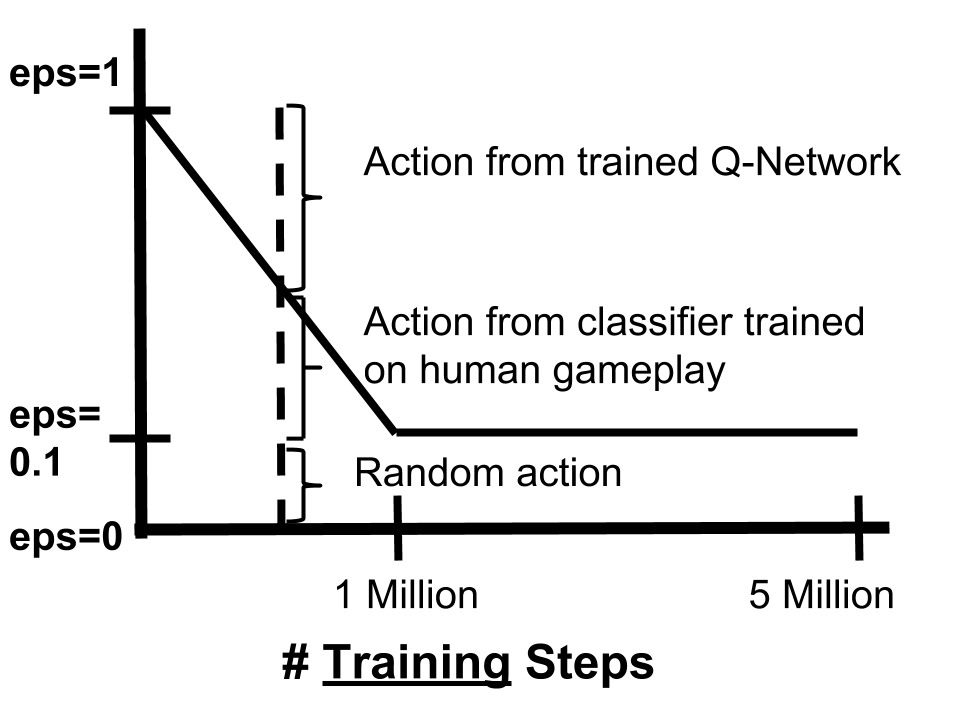
\includegraphics[width=0.45\textwidth]{figures/dqn_with_human_data_graph.png}
\caption{\footnotesize
The overall picture for our Human-Guided DQN algorithm with regards to
$\epsilon$ decay during Q-Learning. During the exploration stage, instead of
playing random actions with probability $\epsilon$, we perform the action chosen
from our trained classifier with probability $\epsilon-0.1$, up until 1 million
steps, upon which time our classifier is ignored. Note that, as described in
Section~\ref{sec:results_p2}, we sometimes adjust the number of steps taken to
investigate the impact of a longer exploration period.
}
\label{fig:human-guided-dqn}
\end{figure}

To ensure sufficient exploration of the state space, both standard Q-Learning
and standard DQN follow $\epsilon$-greedy policies, where the action to take at
state $s$ is selected to be $a = \argmax_a Q(s,a)$ with probability $1-\epsilon$
and randomly selected otherwise. The code from~\cite{mnih-dqn-2015} initializes
at $\epsilon=1.0$ and linearly anneals it down to 0.1 after the first one
million steps, and then fixes it thereafter.

Our objective is to provide potentially better state exploration by utilizing
human data. Rather than choose an action with probability $\epsilon$, which will
be high in the beginning, why not choose the action that a human would take? One
hopeful outcome is that this will ``bias'' the state exploration space towards
``better'' areas, and then standard DQN would continue to build upon that
positive exploration to obtain higher-quality rewards. In particular, we hope to
see that this method provides improvement in the beginning of the exploration
stage relative to standard DQN.

Figure~\ref{fig:human-guided-dqn} presents a picture of the overall pipeline.
During the first million training steps where $\epsilon$ is linearly annealed,
when the agent selects a random action, we usually (but not always) choose
instead the action chosen by the classifier trained on human data. We leave a
fixed probability of $\epsilon=0.1$ to choose random actions, in part because
certain games have actions which appear extremely infrequently (e.g., FIRE in
Breakout during human gameplay occurs around five times per game) but will be
executed via these random actions. We call our method \emph{Human-Guided DQN}.

\subsection{Methodology and Implementation}\label{ssec:implementation}

There are three major steps for the experiments: getting human gameplay,
developing a classifier to map from game frames to actions, and then plugging it
into DQN. 

\subsubsection{Human Gameplay} To enable human gameplay, we modify the Arcade
Learning Environment (ALE)~\cite{bellemare13arcade} to enable a human to play.
Each time step, we save the RGB game screen, the action taken, and the reward
received. The human player is the author of this paper, who is an expert in
Breakout and Space Invaders with roughly twenty hours and eight hours of prior
gampeplay experience for these respective
games.\footnote{In~\cite{mnih-dqn-2015}, human experts had only two hours of
training.} We ultimately collected human gameplay data based on six hours of
Breakout and five hours of Space Invaders. Due to the time-consuming nature of
this work, we leave analysis on other Atari games to future work.

\subsubsection{Developing a Classifier} With the data from the human gameplay,
we apply all the standard preprocessing steps performed in~\cite{mnih-dqn-2015},
such as frame skipping and taking four consecutive (but non-skipped) frames to
form a state. We then build a CNN using the same architecture as the Q-Network
from~\cite{mnih-dqn-2015}, which uses three convolutional layers followed by two
fully connected layers (though we add a softmax at the end to get a
distribution). The network has the number of output nodes equal to the number of
actions chosen, thus allowing all $Q(\phi_i,a_j)$ values to be determined for
all actions $a_j$ during one pass with $\phi_i$ as input.  As mentioned in
Section~\ref{ssec:algorithm}, however, we filter the actions so that those which
are designed to happen extremely infrequently are not considered (instead, they
are played via the random actions or the standard Q-Network in DQN). For Deep
Learning code, we use the Theano library~\cite{2016arXiv160502688short}.  Our
classifier's code and supporting documents are
open-source.\footnote{\url{https://github.com/DanielTakeshi/Algorithmic-HRI}}

\subsubsection{The DQN Algorithm} Upon developing a classifier, we rigorously
tuned it (see Section~\ref{ssec:results_classifier}) to identify the strongest
hyperparameters. We then modified a popular open-source implementation of DQN to
load in the model weights into a new network (but with the same architecture)
and to enable it to use the classifier during the training process. Again, our
code is open-source on
GitHub.\footnote{\url{https://github.com/DanielTakeshi/deep_q_rl}}



%%%%%%%%%%%%%%%%%%%%%%%%%%%%%%%%%%%%%%%%%%%%%%%%%%%%%%%%%%%%%%%%%%%%%%%%%%%%%%%%
\section{Results: Human Gameplay}\label{sec:results_p1}

\subsection{Classifier Performance}\label{ssec:results_classifier}

% Daniel: this was done with Breakout and the CORRECT cropping method,
% fortunately!
\begin{table}[!t]
\renewcommand{\arraystretch}{1.3}
\caption{Tuning Classifiers on Breakout}
\label{tab:breakout}
\centering
\begin{tabular}{c c c c | c c c c}
\hline
Reg.  & $\lambda$ & Train & Valid & Reg.  & $\lambda$ & Train & Valid \\
\hline
$L_1$ & 0.00005   & \textbf{99.2}  & 82.1  & $L_2$ & 0.00005   & \textbf{99.6}  & 83.5 \\
$L_1$ & 0.0001    & 98.9  & 82.2  & $L_2$ & 0.0001    & 99.4  & 83.1 \\
$L_1$ & 0.0005    & 87.6  & \textbf{85.6}  & $L_2$ & 0.0005    & \textbf{99.6}  & 83.2 \\
$L_1$ & 0.001     & 85.0  & 84.4  & $L_2$ & 0.005     & 95.6  & 84.6 \\
$L_1$ & 0.005     & 85.1  & 83.9  & $L_2$ & 0.001     & 99.0  & 83.1 \\
$L_1$ & 0.01      & 77.6  & 76.0  & $L_2$ & 0.01      & 88.3  & \textbf{86.3} \\
$L_1$ & 0.05      & 33.7  & 36.8  & $L_2$ & 0.05      & 84.6  & 84.1 \\
\hline
\end{tabular}
\end{table}

% Whew ... I think these numbers should be all correct.
\begin{table}[!t]
\renewcommand{\arraystretch}{1.3}
\caption{Tuning Classifiers on Space Invaders}
\label{tab:space_invaders}
\centering
\begin{tabular}{c c c c | c c c c}
\hline
Reg.  & $\lambda$ & Train & Valid & Reg.  & $\lambda$ & Train & Valid \\
\hline
$L_1$ & 0.00005   & \textbf{96.3}  & 67.5  & $L_2$ & 0.00005   & \textbf{97.8}  & 66.0 \\
$L_1$ & 0.0001    & 94.7  & 68.2  & $L_2$ & 0.0001    & \textbf{97.8}  & 66.9 \\
$L_1$ & 0.0005    & 76.5  & \textbf{74.5}  & $L_2$ & 0.0005    & 96.5  & 68.4 \\
$L_1$ & 0.001     & 74.4  & 73.4  & $L_2$ & 0.001     & 95.1  & 68.2 \\
$L_1$ & 0.005     & 65.9  & 65.8  & $L_2$ & 0.005     & 81.0  & \textbf{72.7} \\
$L_1$ & 0.01      & 28.5  & 29.0  & $L_2$ & 0.01      & 75.9  & \textbf{72.7} \\
$L_1$ & 0.05      & 28.5  & 29.0  & $L_2$ & 0.05      & 64.7  & 64.0 \\
\hline
\end{tabular}
\end{table}

\begin{figure}[t]
\centering
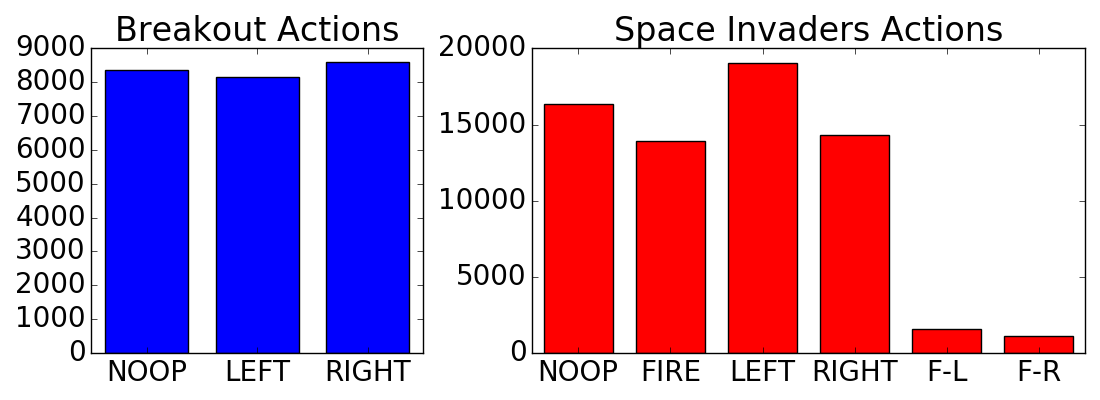
\includegraphics[width=0.48\textwidth]{figures/bar_charts_actions.png}
\caption{\footnotesize
The distribution of actions for Breakout (left) and Space Invaders (right)
within all our data used for classification. This is the distribution obtained
\emph{after} pre-processing steps to eliminate most NOOP actions. For Breakout,
we randomly select $x$ NOOP actions out of the full set, where $x$ is the
average of the LEFT and RIGHT action counts. For Space Invaders, we kept one
third of the NOOP actions. F-L and F-R represent ``FIRE LEFT'' and ``FIRE
RIGHT'', respectively.
}
\label{fig:action_distribution}
\end{figure}

After collecting the human gameplay, we formed a dataset $\mathcal{D}$
consisting of state-action pairs $\mathcal{D}=\{\phi_i, a_i\}_{i=1}^N$
encountered during human gameplay, where $\phi_i$ consists of four $84\times 84$
consecutive (non-skipped) grayscale images $\phi_i =
(s_{i-3},s_{i-2},s_{i-1},s_i)$ and $a_i$ is the action chosen (by the human
player) after observing game frame $s_i$.

During normal human gameplay, the distribution of actions is skewed, presenting
a challenge for training a classifier. In Breakout, the NOOP action tends to be
chosen far more often than LEFT or RIGHT, and the FIRE action is designed to
occur only five times a game. We therefore do not incorporate FIRE in our
Breakout classifier and subsample NOOP actions. For Space Invaders, the FIRE
actions (also including FIRE LEFT and FIRE RIGHT) occur more frequently, so we
included them in the classifier, but still only kept a third of the NOOP
actions.  Thus, Breakout results in a balanced three-way classification task,
while Space Invaders results in a (less-balanced) six-way classification task.
Figure~\ref{fig:action_distribution} shows the action distributions.

As described in Section~\ref{ssec:implementation}, we built a CNN following the
architecture from~\cite{mnih-dqn-2015}. We split the data into training,
validation, and testing sets, and tuned weights via either $L_1$ or $L_2$
regularization based on validation set performance.\footnote{In this setting, it
is probably OK to tune on the test set, but we decided to stick to best
practices and tune on the validation set. For both games, the best-performing
settings on the validation set also corresponded to the top settings for the
test sets.}

Tuning results are shown in Tables~\ref{tab:breakout}
and~\ref{tab:space_invaders}, with bold indicating the best settings. With low
$\lambda$, the net gets arbitrarily high performance on the training data, but
performs poorly otherwise. For both games, we keep only the best-performing net
on the validation set. In Breakout, the best net achieves 86.3\% accuracy on the
validation set, and for Space Invaders, that figure is 74.5\%, which is lower
due to the more challenging classification task. The per-class results on the
\emph{test} set are shown in Tables~\ref{tab:breakout_perclass}
and~\ref{tab:spaceinv_perclass}, respectively. The results indicate that all
three actions are fairly easy to detect for Breakout, but for Space Invaders,
our classifiers are better at detecting LEFT and RIGHT actions.

\subsection{Classifier Investigation}

% More tables, this time for the action distribution!
\begin{table}[!t]
\renewcommand{\arraystretch}{1.3}
\caption{Per-Class Performance on Breakout}
\label{tab:breakout_perclass}
\centering
\begin{tabular}{c c c c}
\hline
        & NOOP  & LEFT & RIGHT \\
\hline
Correct & 1463 & 1492 & 1390 \\
Total   & 1635 & 1784 & 1605 \\
Percent & 89.4 & 83.6 & 86.6 \\
\hline
\end{tabular}
\end{table}

% Same thing this time for SI
\begin{table}[!t]
\renewcommand{\arraystretch}{1.3}
\caption{Per-Class Performance on Space Invaders}
\label{tab:spaceinv_perclass}
\centering
\begin{tabular}{c c c c c c c}
\hline
        & NOOP & FIRE & LEFT & RIGHT & F-L  & F-R  \\
\hline
Correct & 2255 & 1660 & 2462 & 3378  &  34  &   83 \\
Total   & 3310 & 2699 & 2817 & 3870  &  246 &  306 \\
Percent & 68.1 & 61.5 & 87.3 & 87.2  & 13.8 & 27.1 \\
\hline
\end{tabular}
\end{table}


\begin{figure*}[t]
\centering

\includegraphics[width=0.30\textwidth]{figures/empty.png}
\caption{\footnotesize
Four examples of ``states'' $\phi_t = (s_{t-3},s_{t-2},s_{t-1},s_t)$ encountered
during human gameplay, two for Breakout (left) and two for Space Invaders
(right). Top left: the action XXX is correctly predicted (XXX confidence).
Bottom left: the action XXX is correctly predicted (XXX confidence). Top right:
the action XXX is correctly predicted (XXX confidence). Bottom right: the action
XXX is correctly predicted (XXX confidence).
}
\label{fig:example_game_frames}
\end{figure*}

We further investigate the top-performing Breakout and Space Invaders classifier
by visually inspecting example outputs. Figure~\ref{fig:example_game_frames}
demonstrates examples of two states $\phi$ for each of the two games, where the
classifier (correctly) predicted the action the human player took with high
confidence (as determined by the softmax probability distribution).

In Breakout, we see that ...

In Space Invaders, ...




%%%%%%%%%%%%%%%%%%%%%%%%%%%%%%%%%%%%%%%%%%%%%%%%%%%%%%%%%%%%%%%%%%%%%%%%%%%%%%%%
\section{Results: Modified DQN}\label{sec:results_p2}

\begin{figure*}[t]
\centering

\includegraphics[width=0.30\textwidth]{figures/empty.png}
\caption{\footnotesize
Plots which compare the performance of standard DQN (black) versus Human-Guided
DQN (blue) on Breakout (first two subplots) and Space Invaders (last two
subplots). The metrics used are the average reward obtained per episode
and the average $Q$-value encountered during gameplay. Since the outcome is
extremely noisy, the reward per episode is a smoothed version, computed with
$avg = 0.7\cdot avg + 0.3\cdot newscores$.
}
\label{fig:human_dqn_performance}
\end{figure*}

\begin{figure}[t]
\centering

\includegraphics[width=0.30\textwidth]{figures/empty.png}
\caption{\footnotesize
A comparison of the rewards obtained via standard DQN (black) versus
Human-Guided DQN (blue) on Space Invaders. This is similar to the Space Invaders
subplots of Figure~\ref{fig:human_dqn_performance}, except that the exploration
period is 10x longer and the number of epochs has been reduced from 200 to 80.
(The exploration phase ``ends'' after epoch 40, which is when $\epsilon=0.1$.)
}
\label{fig:sp_inv_longer_exploration}
\end{figure}

TODO

We ran our experiments on a single computer with an NVIDIA TITAN GPU (with
Pascal).

TODO

Figure~\ref{fig:human_dqn_performance}

One factor which hinders the previous analysis\footnote{This was due to some
extra settings inside the open source DQN code which were not obvious at first
glance.} is that the exploration period is likely too short for us to discern
any noticeable improvements. The exploration period consists of when
$\epsilon>0.1$, and for the previous settings, that ends after the fourth of 200
epochs. This does not give us enough data points, so we re-ran the Space
Invaders experiment using an exploration period 10x longer. Due to computational
limitations, we limited the runs to 80 epochs total.

Figure~\ref{fig:sp_inv_longer_exploration} shows the results with the improved
experiment settings. \textbf{TODO ANALYSIS}




%%%%%%%%%%%%%%%%%%%%%%%%%%%%%%%%%%%%%%%%%%%%%%%%%%%%%%%%%%%%%%%%%%%%%%%%%%%%%%%%
\section{Conclusions}\label{sec:conclusions}

In this work, we have made efforts to use Learning from Demonstration techniques
to boost the performance of DQN agents on Atari games. We collected many hours
of human expert gameplay data on Breakout and Space Invaders, and provided
evidence that a CNN can largely predict the human expert's actions. Our
Human-Guided DQN utilized this classifier for exploration. Unfortunately, the
results did not substantially improve, but we believe there is still untapped
potential in this project. In future work, we will run Human-Guided DQN with
longer exploration phases. Second, we will try using \emph{human experience
replay}: combining the usual experience replay with subsampled human gameplay
data. Finally, a more elaborate goal is to work on training attention
models~\cite{NIPS2014_5542,icml2015_xuc15}, the idea being that for these games,
there are only a few important signals that matter for rewards, and this can be
trained into an attention model, which hopefully can be used to improve DQN
performance.

\bibliographystyle{abbrv}
\bibliography{Daniel_Seita_Report_AHRI}
\end{document}
